\vspace{-0.25em}
\section{Experimental Evaluation}
\label{sec:evaluation}
\vspace{-0.25em}

We evaluate our Gdev prototype, using the Rodinia
benchmarks~\cite{Che_IISWC09}, GPU-accelerated eCryptfs encrypted
filesystem from KGPU~\cite{Sun_SECURITY11_Poster}, FAST database
search~\cite{Kim_SIGMOD10}, and some dataflow
microbenchmarks from PTask~\cite{Rossbach_SOSP11}.
We disclose that the basic performance of our prototype is practical
even compared to proprietary software, and also demonstrate that Gdev
provides significant benefits for GPU applications in time-sharing
systems.

Our experiments are conducted with the Linux kernel 2.6.39 on NVIDIA
GeForce~GTX~480 graphics card and Intel Core~2~Extreme QX9650 processor.
GPU programs are written in CUDA and compiled by NVCC~\cite{CUDA40},
while CPU programs are compiled by gcc 4.4.6.

\vspace{-0.25em}
\subsection{Basic Performance}
\vspace{-0.25em}

\begin{figure}[t]
 \begin{center}
  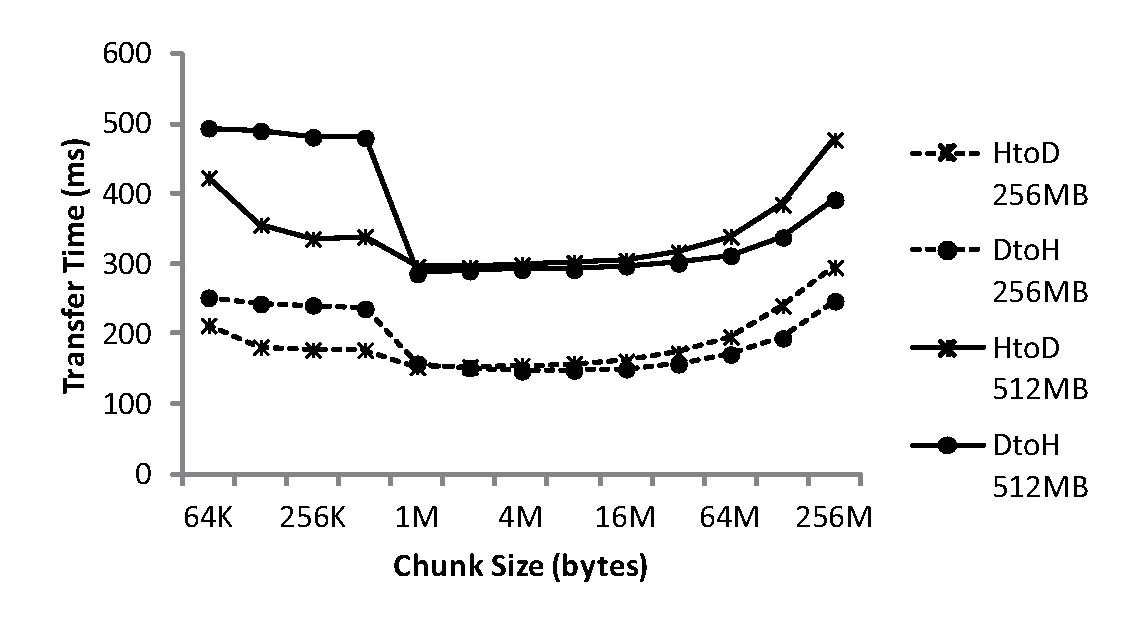
\includegraphics[width=0.8\hsize]{eps/chunk.eps}\\
  \vspace{-1.5em}
  \caption{Impact of the chunk size on DMA speeds.}
  \label{fig:chunk}
 \end{center}
 \vspace{-1.5em}
 \begin{center}
  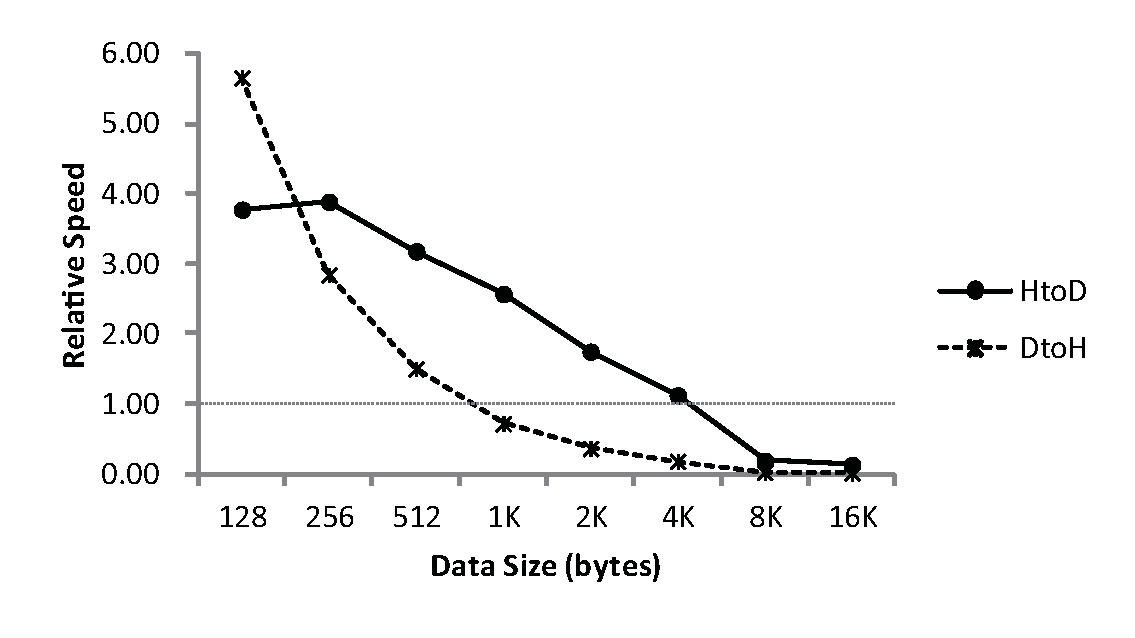
\includegraphics[width=0.8\hsize]{eps/dma.eps}\\
  \vspace{-1.5em}
  \caption{Relative speed of I/O access to DMA.}
  \label{fig:io_access}
 \end{center}
 \vspace{-1.5em}
 \begin{center}
  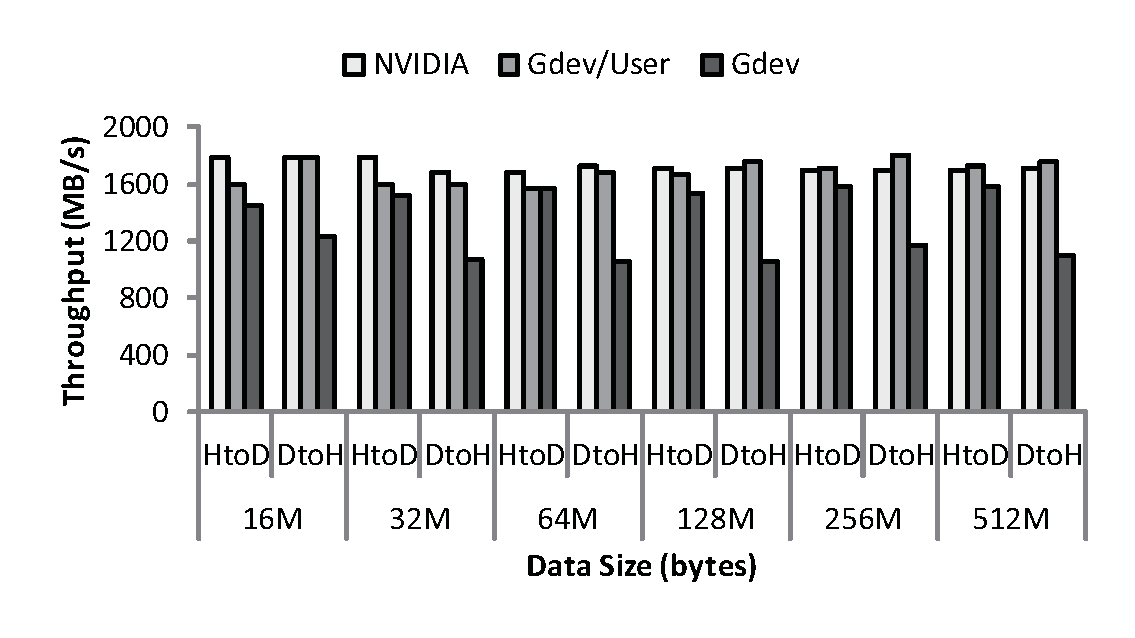
\includegraphics[width=0.9\hsize]{eps/memcpy.eps}\\
  \vspace{-1.5em}
  \caption{Memory-copy throughput.}
  \label{fig:memcpy}
 \end{center}
 \vspace{-1.5em}
\end{figure}

We evaluate the standalone performance of applications achieved by
our Gdev prototype to argue that the rest of our evaluation is practical
in the real world.
To this end, first of all, we need to find the best parameters used for
memory-copy optimization, using simple test code that copies data
between device and host memory.

Figure~\ref{fig:chunk} shows the impact of the chunk size on data
transfer times for host-to-device (HtoD) and device-to-host (DtoH)
directions respectively, when using DMA-based memory-copy operations
with 256MB and 512MB of data.
Since each chunk incurs some overhead in DMA configuration, a
smaller chunk size producing a greater number of chunks increases a
transfer time.
On the other hand, there is a constraint that the first and last pieces
of chunks cannot be overlapped with others, as described in
Section~\ref{sec:memory_copy}.
Hence, a larger chunk size leading to a longer blocking time with these
pieces of chunks also increases a transfer time.
According to our observation, a chunk size of 4MB is the best trade-off
for both HtoD and DtoH directions.
We therefore set the chunk size to 4MB for our experiments.

Figure~\ref{fig:io_access} shows the relative speed of direct I/O
access to DMA for a small size of data. 
Due to some hardware effect, HtoD and DtoH directions show different
transfer times, but it clearly explains the advantage of direct I/O
access for small data.
According to our observation, the data transfer speed inverses around a
data size of 4KB and 1KB for HtoD and DtoH directions respectively.
We therefore set the boundary of direct I/O access and DMA to 4KB and
1KB for them respectively.

Figure~\ref{fig:memcpy} shows memory-copy throughput achieved
by our Gdev prototype compared to NVIDIA's proprietary software.
``Gdev/User'' employs a runtime library in the user-space, while
``Gdev'' integrates runtime support into the OS.
Interestingly, user-space runtime achieves higher throughput than
OS-space runtime, particularly for DtoH direction.
This difference comes from \texttt{memcpy}'s effect within host memory.
In fact, the \texttt{memcpy} implementation in the Linux kernel is slower
than that in the user-space GNU library, when copying data from host I/O
to main memory.
This could be a disadvantage of our approach.
We will investigate this effect more in depth.
Apart from the DtoH memory-copy throughput, however, our Gdev prototype
and NVIDIA's proprietary software are almost competitive.
 
\begin{table}[t]
 \caption{List of benchmarks.}
 \label{tab:benchmarks}
 \vspace{-0.5em}
 \begin{center}
  {\footnotesize
  \begin{tabular}{|l|l|}
   \hline
   \textbf{Benchmark} & \textbf{Description}\\
   \hline
   LOOP & Long-loop compute without data \\
   \hline
   MADD & 1024x1024 matrix addition\\
   \hline
   MMUL & 1024x1024 matrix multiplication\\
   \hline
   CPY & 256MB of HtoD and DtoH\\
   \hline
   PINCPY & CPY using pinned host I/O memory\\
   \hline
   BP & Back propagation (pattern recognition)\\
   \hline
   BFS & Breadth-first search (graph algorithm)\\
   \hline
   HW & Heart wall (medical imaging)\\
   \hline
   HS & Hotspot (physics simulation)\\
   \hline
   LUD & LU decomposition (linear algebra)\\
   \hline
   NN & K-nearest neighbors (data mining)\\
   \hline
   NW & Needleman-wunsch (bioinformatics)\\
   \hline
   SRAD & Speckle reducing anisotropic diffusion (imaging)\\
   \hline
   SRAD2 & SRAD with random pseudo-inputs (imaging)\\
   \hline
  \end{tabular}
  }
 \end{center}
 \vspace{-1.5em}
\end{table}

Figure~\ref{fig:basic_performance} demonstrates the standalone
performance of benchmarks achieved by our Gdev prototype compared to
NVIDIA's proprietary software.
Table~\ref{tab:benchmarks} describes the microbenchmarks and
Rodinia~\cite{Che_IISWC09} benchmarks used in this evaluation.
First of all, we have found that NVIDIA GPUs have some ``performance
mode'' to boost hardware performance that we do not use for our Gdev
prototype implementation.
As observed in the LOOP benchmark result, our Gdev prototype incurs
about 20\% of decrease in performance compared to the proprietary
software due to a lock of performance mode.
However, the impact of performance mode is workload dependent.
If workloads are very compute-intensive, such as the HW and SRAD
benchmarks, this impact appears clearly, whereas some friendly workloads,
such as the BFS and HS benchmarks, can hide this impact.
In either case, however, this is an implementation issue, but is
not a conceptual limitation of Gdev.
These benchmark results also imply that Gdev's runtime-unified OS approach
is not appreciated by data-intensive workloads.
For example, the BP benchmark deals with a very large size of data,
though its compute demand is not very high.
Such a workload would not perform well with our Gdev prototype, since
the \texttt{memcpy} implementation in the Linux kernel is slow.
On the other hand, the PINCPY benchmark shows little difference in
performance for our Gdev prototype and the proprietary software, since
it does not need \texttt{memcpy} operations.

\begin{figure}[t]
 \begin{center}
  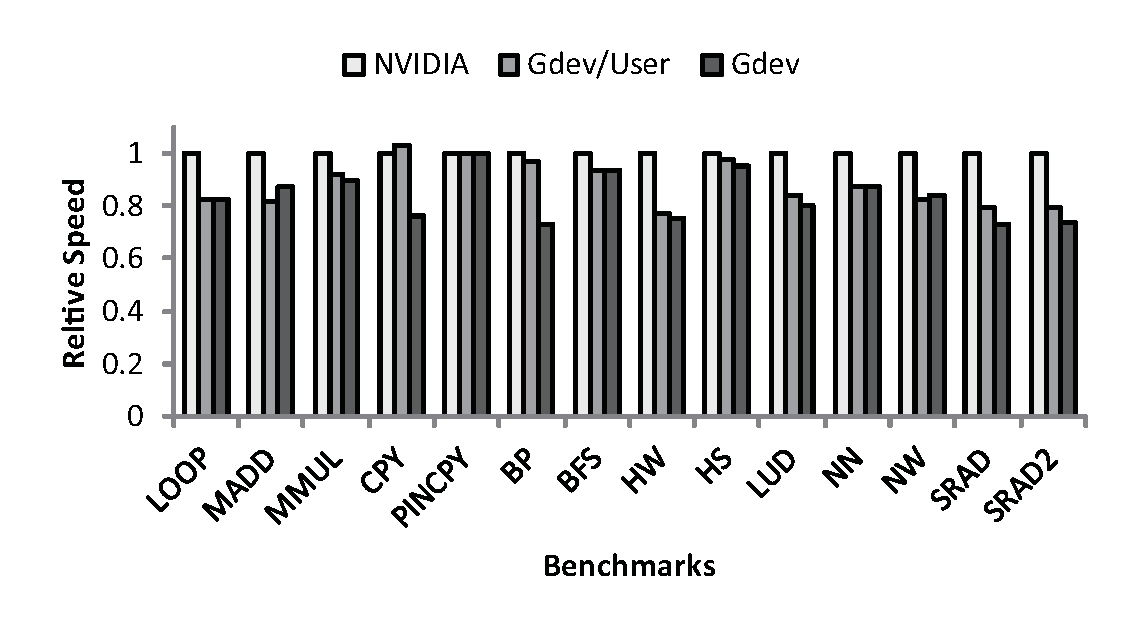
\includegraphics[width=0.9\hsize]{eps/basic_performance.eps}\\
  \vspace{-1.5em}
  \caption{Basic standalone performance.}
  \label{fig:basic_performance}
 \end{center}
 \vspace{-1.5em}
 \begin{center}
  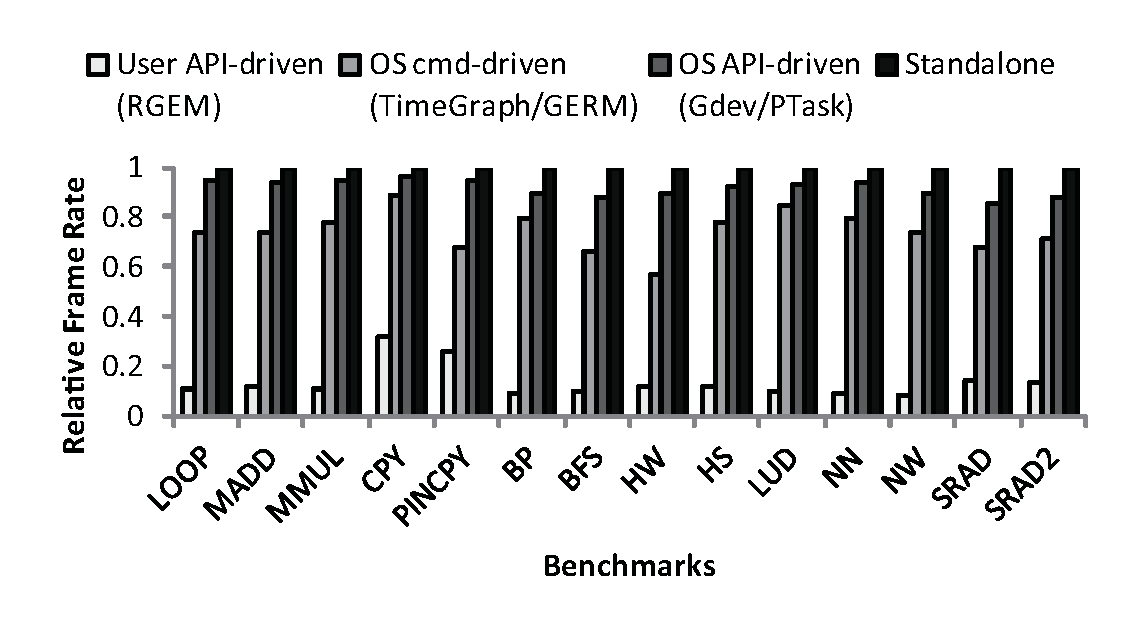
\includegraphics[width=0.9\hsize]{eps/scheduler_overhead.eps}\\
  \vspace{-1.5em}
  \caption{Unconstrained real-time performance.}
  \label{fig:scheduler_overhead}
 \end{center}
 \vspace{-1.5em}
\end{figure}

\vspace{-0.25em}
\subsection{Reliability}
\vspace{-0.25em}

We next evaluate reliability of OS-space runtime support by comparing
the OS-space API-driven scheme adopted by Gdev and
PTask~\cite{Rossbach_SOSP11}, OS-space command-driven scheme adopted by
TimeGraph~\cite{Kato_ATC11} and GERM~\cite{Bautin_MCNC08}, and
user-space API-driven scheme adopted by RGEM~\cite{Kato_RTSS11}.
We execute Rodinia benchmarks recursively as fast as possible in
real-time, contending with such a programs that bypasses the user-space
runtime library and launch many meaningless GPU computations.
The user-space API-driven scheme severely suffers from this
situation, since it cannot schedule such a bypassing program at all.
The OS-space command-driven scheme can sustain the contention to some
extent by the command scheduler, but the overhead becomes non-trivial
due to many scheduler invocations.
The OS-space API-driven scheme, on the other hand, can reject such a
bypassing program, since it is not submitted through the API.
Gdev and PTask are both API-driven, but PTask exposes the system call to
the user space, such as \texttt{sys\_set\_ptask\_prio}, 
which could allow misbehaving programs to abuse GPU priorities.
As a consequence, Gdev's approach that integrates runtime support into
the OS is a more reliable solution.

\vspace{-0.25em}
\subsection{GPU Acceleration for the OS}
\vspace{-0.25em}

\begin{figure}[t]
 \begin{center}
  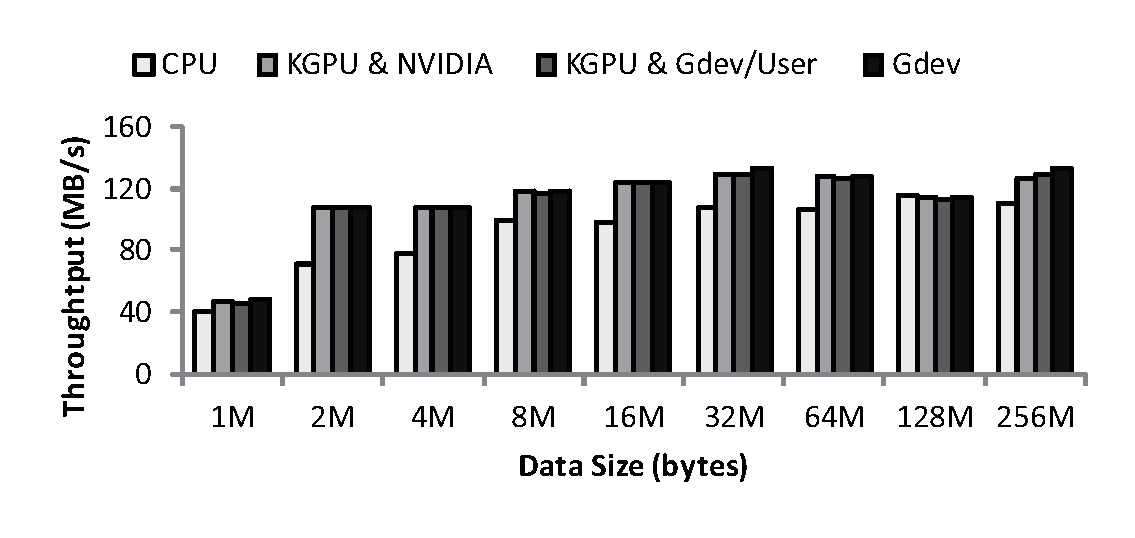
\includegraphics[width=0.9\hsize]{eps/ecryptfs_read.eps}\\
  \vspace{-1.5em}
  \caption{eCryptfs read throughput.}
  \label{fig:ecryptfs_read}
 \end{center}
 \vspace{-1.5em}
 \begin{center}
  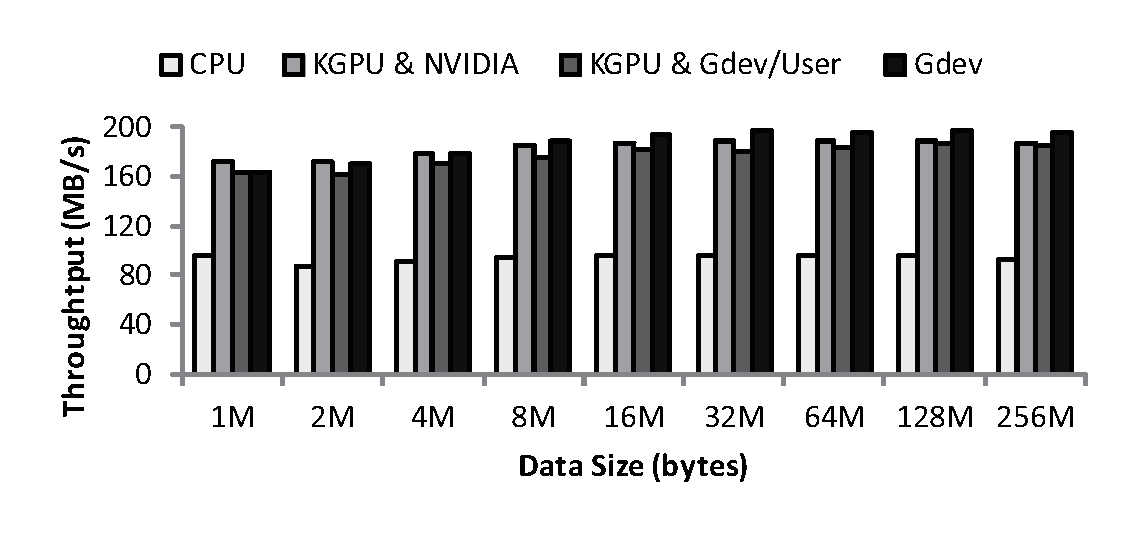
\includegraphics[width=0.9\hsize]{eps/ecryptfs_write.eps}\\
  \vspace{-1.5em}
  \caption{eCryptfs write throughput.}
  \label{fig:ecryptfs_write}
 \end{center}
 \vspace{-1.5em}
 \begin{center}
  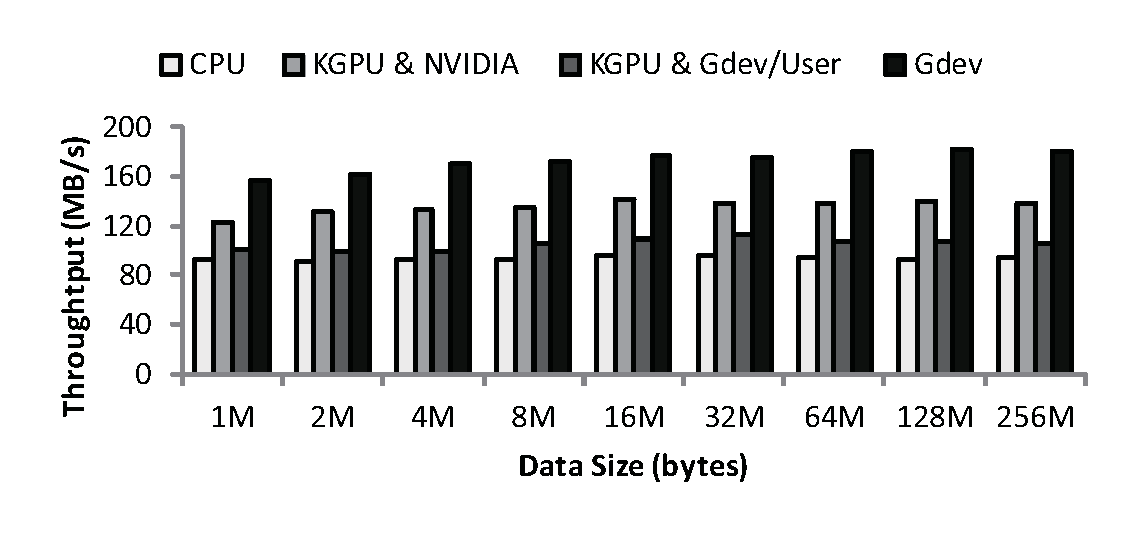
\includegraphics[width=0.9\hsize]{eps/ecryptfs_write_multitask.eps}\\
  \vspace{-1.5em}
  \caption{eCryptfs write throughput with priorities.}
  \label{fig:ecryptfs_write_multitask}
 \end{center}
 \vspace{-1.5em}
\end{figure}

We now evaluate the performance of the Linux encrypted file system
accelerated by the GPU.
In particular, we use KGPU's implementation of
eCryptfs~\cite{Sun_SYSTOR12}.
KGPU is a framework that allows the OS to access the user-space runtime
library to use GPUs for computations.
We have modified KGPU's eCryptfs implementation to call the CUDA API
functions provided by Gdev directly instead of sending requests to the
KGPU user-space daemon.

Figure~\ref{fig:ecryptfs_read} and \ref{fig:ecryptfs_write} show the
read and write throughput of several versions of eCryptfs.
``CPU'' represents the CPU implementation, while ``KGPU \& NVIDIA'' and
``KGPU \& Gdev/User'' represent those using KGPU with NVIDIA's library
and Gdev's library respectively in the user space. 
``Gdev'' is our contribution that enables the eCryptfs module to use the
GPU directly within the OS.
Due to some page cache effect, read and write are not identical in
throughput, but an advantage of using the GPU is clearly observed.
One may observe that Gdev's runtime-unified OS approach does not really
outperform KGPU's approach.
This is not surprising at all, because a magnitude of improvements in
latency achieved by our OS approach would be at most microseconds, while
the AES/DES operations of eCryptfs performed on the GPU are
orders-of-milliseconds.
Nonetheless, Gdev provides a significant benefit that the OS is freed
from the user space, and thus is more secure.

A further advantage of using Gdev appears in a multi-tasking scenario.
Figure~\ref{fig:ecryptfs_write_multitask} shows the write throughput of
eCryptfs when the FAST search task~\cite{Kim_SIGMOD10} is competing for
the GPU.
Since Gdev supports priorities in the OS, we can assign the eCryptfs
task with the highest priority, while the search task is still assigned
a higher priority than other tasks.
Using KGPU in this scenario, however, the performance of eCryptfs is
affected by the search task due to a lack of prioritization, as observed
in ``KGPU \& NVIDIA''.
Even with priorities, KGPU could suffer from a priority inversion
problem, where the high-priority eCryptfs task is reduced to the KGPU
priority level when accessing the GPU, while the search task is
executing at the higher priority level.
We could assign a high priority to the user-space KGPU daemon to avoid
this priority inversion problem, but it affects all user-space GPU
applications performance. 
On the other hand, Gdev can assign each GPU application with an
identical priority, which addresses the priority inversion problem
fundamentally.

\vspace{-0.25em}
\subsection{Impact of Shared Memory}
\vspace{-0.25em}

\begin{figure}[t]
 \begin{center}
  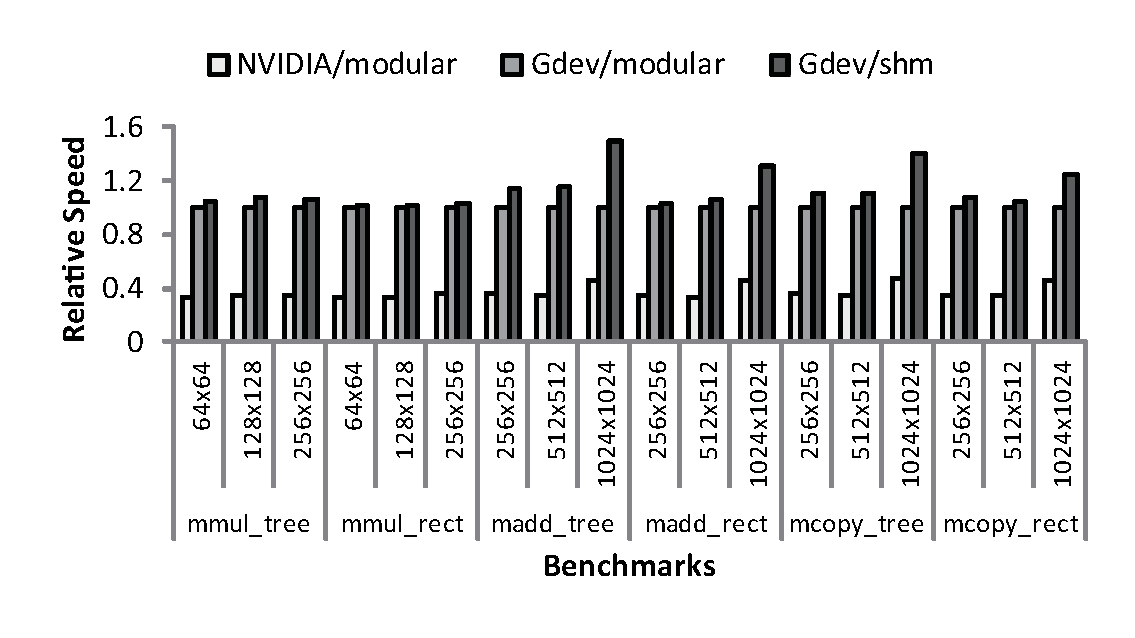
\includegraphics[width=\hsize]{eps/dataflow.eps}\\
  \vspace{-1.5em}
  \caption{Impact of shared memory on dataflow tasks.}
  \label{fig:dataflow}
 \end{center}
 \vspace{-1.5em}
 \begin{center}
  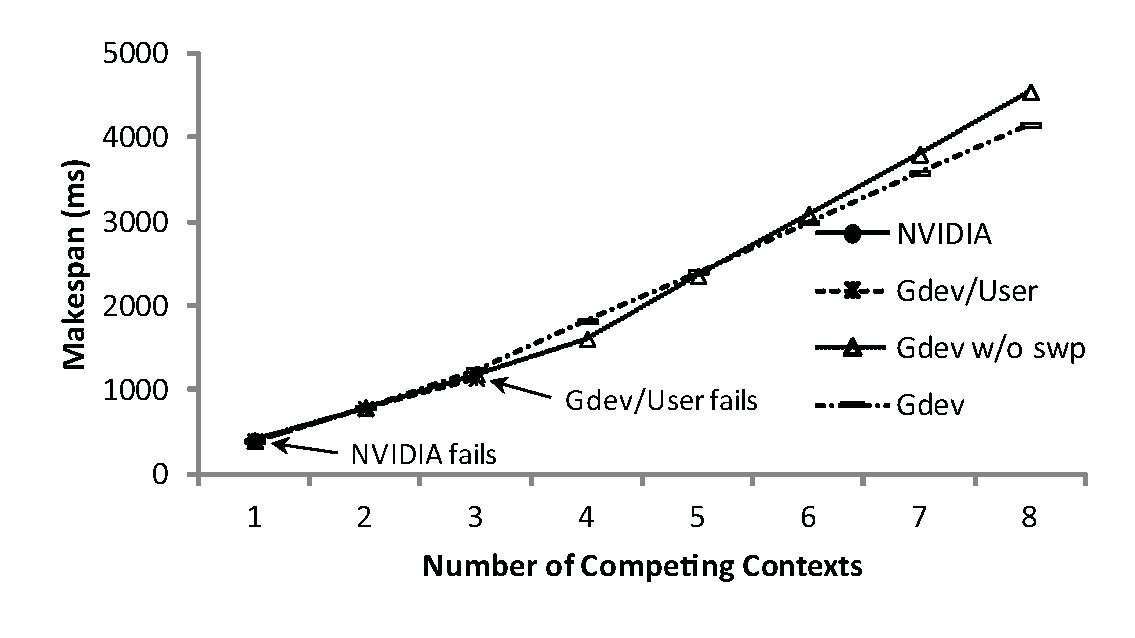
\includegraphics[width=0.75\hsize]{eps/swapping.eps}\\
  \vspace{-1.5em}
  \caption{Impact of swapping latency.}
  \label{fig:swapping}
 \end{center}
 \vspace{-1.5em}
 \begin{center}
  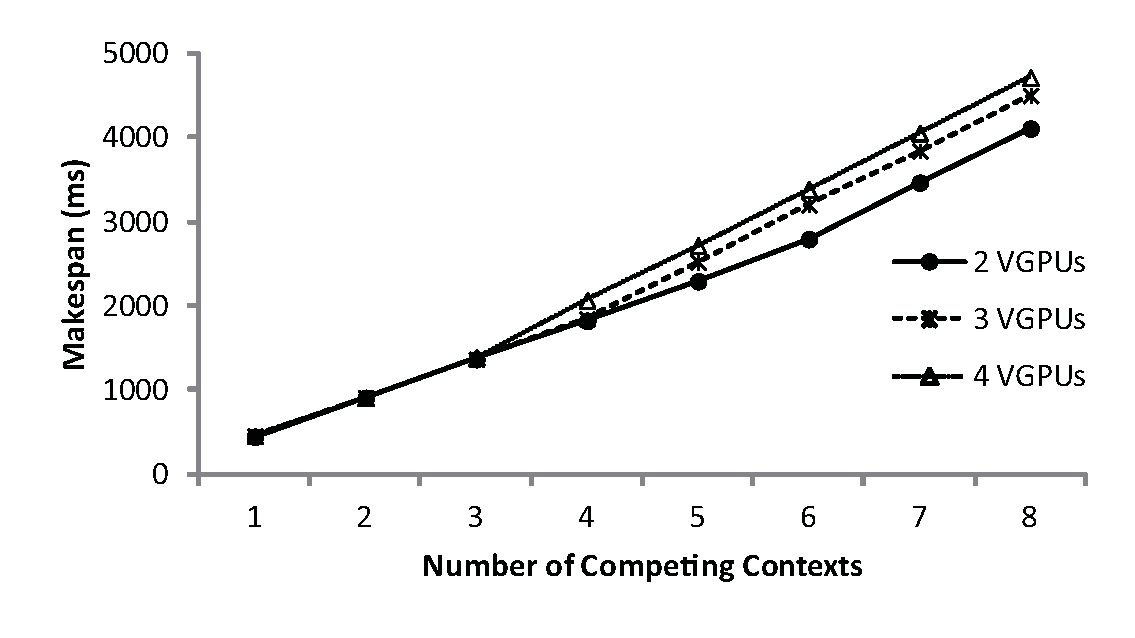
\includegraphics[width=0.75\hsize]{eps/swapping_vgpu.eps}\\
  \vspace{-1.5em}
  \caption{Impact of swapping latency on virtual GPUs.}
  \label{fig:swapping_vgpu}
 \end{center}
 \vspace{-1.5em}
\end{figure}

\begin{figure*}[t]
 \begin{center}
  \subfigure[FIFO scheduler] {
  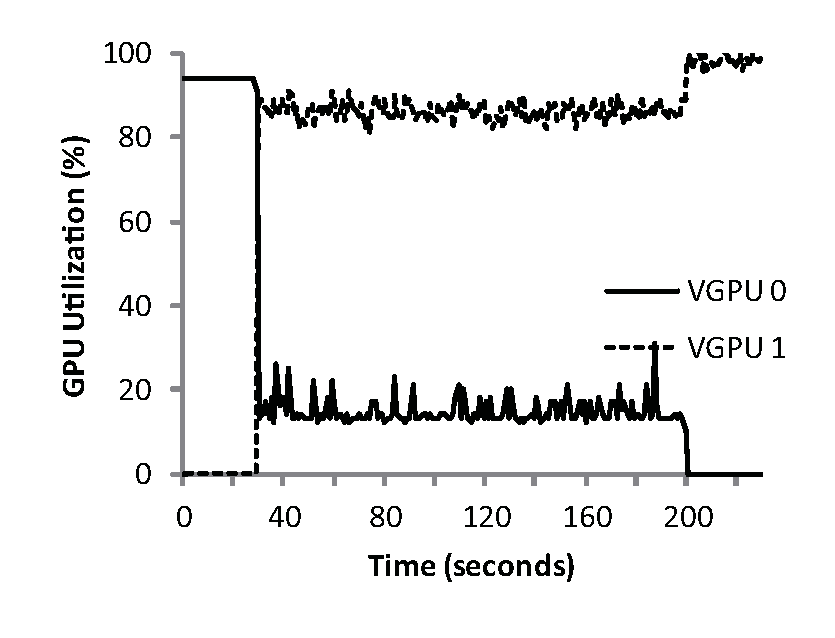
\includegraphics[width=0.319\hsize]{eps/vgpu_2_fifo.eps}
  }
  \subfigure[Credit scheduler] {
  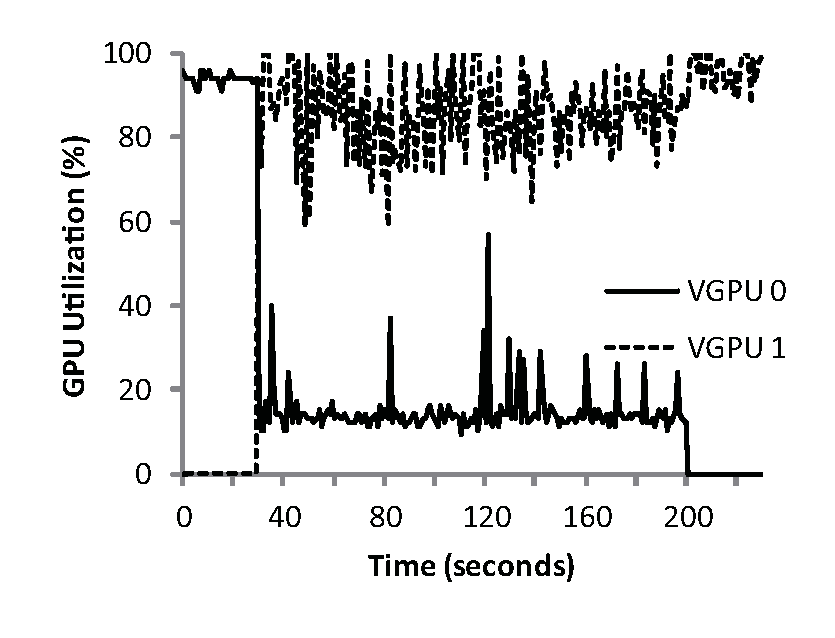
\includegraphics[width=0.319\hsize]{eps/vgpu_2_credit.eps}
  }
  \subfigure[BAND scheduler] {
  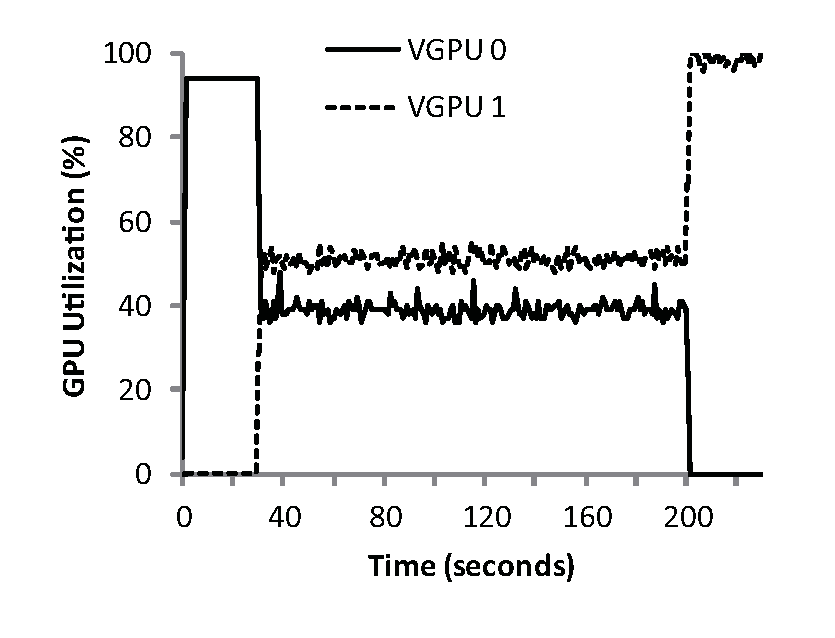
\includegraphics[width=0.319\hsize]{eps/vgpu_2_band.eps}
  }
  \vspace{-1.2em}
  \caption{Util. of virtual GPUs under unfair workloads.}
  \label{fig:vgpu_2}
  \end{center}
  \vspace{-1.5em}
\end{figure*}

Figure~\ref{fig:dataflow} shows the speedups of dataflow benchmarks
brought by Gdev's shared memory scheme.
We construct a dataflow by a 6x32 tree or a 6x10 rectangle, respecting
PTask's setup~\cite{Rossbach_SOSP11}.
``NVIDIA/modular'' and ``Gdev/modular'' use NVIDIA's CUDA API and Gdev's
CUDA API respectively to implement a dataflow in such a way that
allocates a self-contained context to each graph node as a module, and
connects their output and input by copying data between the host and
device memory back and forth.
On the other hand, ``Gdev/shm'' uses shared memory instead of
host-to-device data communication, \textit{i.e.}, it connects the output
and input by sharing the same ``key'' associated with the corresponding
shared memory.
According to the results, the usage of shared memory is very effective
for dataflows with a large size of data, \textit{e.g.}, it gains a 49\%
speedup for the 1024x1024 madd tree.
Specifically, we have observed that ``Gdev/modular'' took 1424ms while
``Gdev/shm'' took 953ms to complete this dataflow.
This makes sense, \textit{i.e.}, the data transfer time for each
1024x1024 integer value was about 8ms on average, and we can reduce data
communications by a total of 32+16+8+4+2=62 intermediate nodes for a
6x32 tree, which leads to a total reduced time of 8x62=496ms.
It should be noted that PTask achieves more speedups due to advanced
dataflow scheduling~\cite{Rossbach_SOSP11}.
However, we provide users with a first-class API primitive for shared
memory, which could be used as a generic IPC method in different program
domains.
Therefore, we distinguish our contribution from PTask.
It is also surprising that our Gdev prototype performs much better than
the proprietary software.
We suspect that the proprietary one takes a long time to initialize
contexts when there are many active contexts, though an in-depth
investigation is required.

Figure~\ref{fig:swapping} depicts the impact of memory swapping,
provided by Gdev, on the makespan of multiple 128MB-data FAST search
tasks, where another 1GB-data FAST search task is running at the highest
priority level.
Given that the GPU used in this evaluation supports
1.6GB of device memory, we cannot create more than three 128MB-data
search tasks at once without memory swapping.
``Gdev/User'' hence fails when the number of the small search tasks
exceeds three, since our prototype does not support shared memory in the
user space.
NVIDIA' proprietary software also fails much earlier.
We suspect that it would reserve a large space of device memory for
other purposes.
With memory swapping, however, all the 128MB-data search tasks can
survive to execute under this memory pressure, though the slope of
increase in the makespan changes at a different point when using the
temporal swap space on the device memory under Gdev.
In particular, a reflection point appears clearly when the device swap
space is not leveraged, as observed in ``Gdev w/o swp'', because the
swapping latency influences the makespan.
Using the device swap space, however, Gdev can reduce the impact of
swapping on the makespan, though a reflection point appears a little
earlier due to the swap space itself causing a less total amount of
device memory available for applications.

Figure~\ref{fig:swapping_vgpu} shows the impact of memory swapping on
virtual GPUs.
In this experiment, we introduce virtual GPUs, and execute 128MB-data
search tasks on the first virtual GPU.
The memory size available for the virtual GPU is more restricted in
the presence of more virtual GPUs.
We confirm that the makespans become longer and their reflection points
appear earlier for a greater number of virtual GPUs, but all the search
tasks can still complete.
This explains that memory swapping is also useful on virtual GPUs.

\vspace{-0.25em}
\subsection{Isolation among Virtual GPUs}
\vspace{-0.25em}

We now examine Gdev's virtual GPU support.
Figure~\ref{fig:vgpu_2} shows the actual GPU utilization of two virtual
GPUs, where the first virtual GPU (VGPU 0) executes short-length compute
programs using the LUD benchmark, while the other (VGPU 1) executes
long-length compute programs using the HW benchmark.
These programs run repeatedly to impose high workloads for 200 seconds
VGPU~1 starts workloads 30 seconds later than VGPU~0.
We compare three schedulers, using the SDQ scheme.
The FIFO scheduler represents a lack of virtual GPU support, and
the Credit scheduler adopts the scheduling policy of the Xen
hypervisor.
The BAND scheduler is one provided by Gdev.
According to the results, the FIFO scheduler does not respect isolation
at all by definition.
The Credit scheduler also does not really work due to unawareness of
non-preemptive burst workload.
The BAND scheduler, however, can provide fairer GPU bandwidth allocations.
The difference between the utilization of two virtual GPUs is retained
within 7\% on average.

We next study the effectiveness of the MRQ scheme that separates the
queues for compute and memory-copy operations.
Figure~\ref{fig:vgpu_2_band_mrq} illustrates the utilization of two
virtual GPUs under the BAND scheduler, executing the SRAD benchmark
tasks with different sizes of image.
We noticed that the compute and memory-copy operations can be
overlapped, but they affect the run-to-completion time with each other.
When VGPU 1 uses more compute resources due to a large size of
computation, the length of memory-copy operations requested by VGPU 0 is
prolonged due to overlapping.
As a result, it requires more memory-copy bandwidth.
However, the available bandwidth is capped by the BAND scheduler,
\textit{i.e.}, both the compute and memory-copy operations are limited 
to about 50\% of bandwidth at most.
One can also observe that the MRQ scheme allowed the sum of compute and
memory-copy bandwidth to exceed 100\%.

We finally demonstrate the scalability of our virtual GPU support.
Figure~\ref{fig:vgpu_fair_4_band} shows the utilization of four virtual
GPUs under the BAND scheduler, where all virtual GPUs execute four
instances of the LUD benchmark task exhaustively to produce fair
workloads.
The workloads of each virtual GPU begin in turn at an interval of 30
seconds.
Under such sane workloads, our virtual GPU support can provide fair
bandwidth allocations, even if the system exhibits non-preemptive burst
workloads.

\begin{figure}[t]
 \begin{center}
  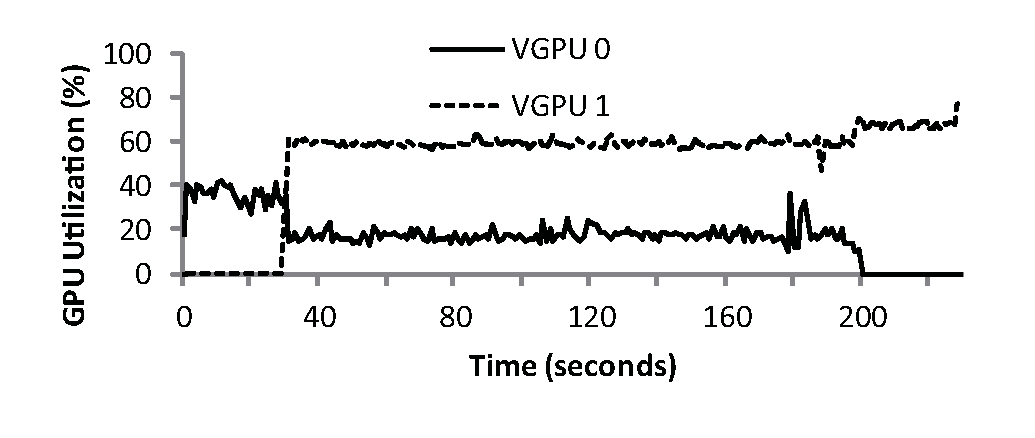
\includegraphics[width=0.9\hsize]{eps/vgpu_2_band_compute.eps}\\
  \vspace{-0.5em}
  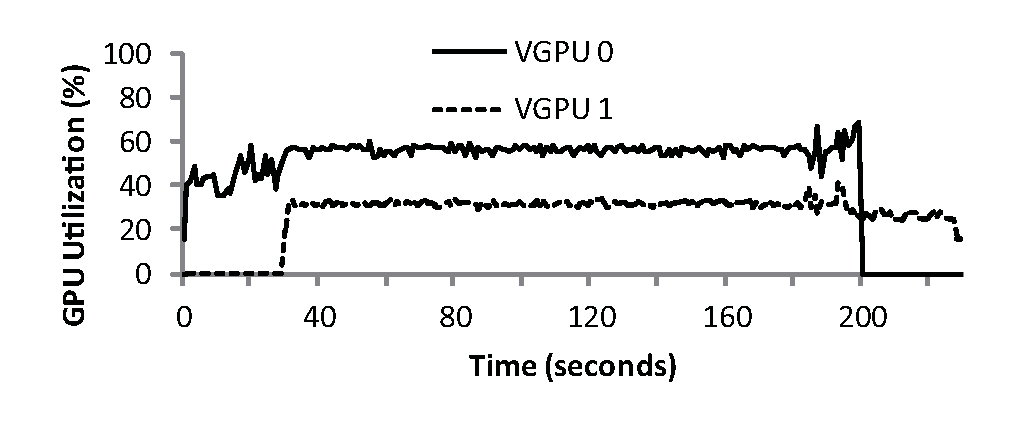
\includegraphics[width=0.9\hsize]{eps/vgpu_2_band_memory.eps}\\
  \vspace{-1.5em}
  \caption{Util. of virtual GPUs with the MRQ scheme (upper for compute
  and lower for memory-copy).}
  \label{fig:vgpu_2_band_mrq}
 \end{center}
 \begin{center}
  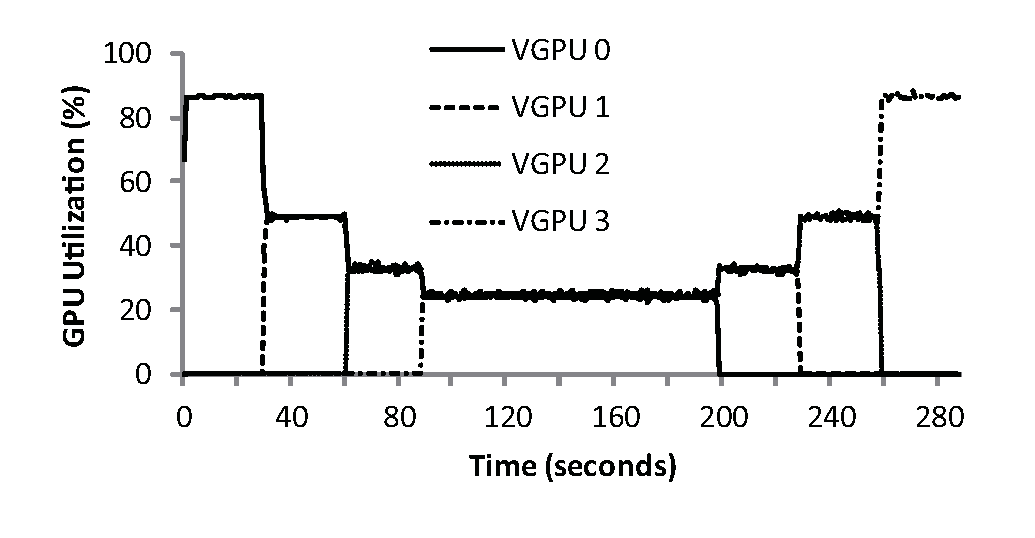
\includegraphics[width=0.9\hsize]{eps/vgpu_fair_4_band.eps}\\
  \vspace{-1.5em}
  \caption{Util. of virtual GPUs under fair workloads.}
  \label{fig:vgpu_fair_4_band}
 \end{center}
  \vspace{-1.5em}
\end{figure}
